\chapter{Protocol Implementation}
\label{chap:protocolimplementation}

This chapter details the simulation environment where the presented High Configurable Protocol was developed and tested. Simulation was chosen 
instead of analytical study or real networks, because this are difficult or expensive for such a complex protocol. During this chapter a 
deeper view into the protocol will be given, as all generated code will be explained in detail.

\section{Used Tools}

To develop this project different simulators and frameworks were considered, choosing finally \ac{OMNeT++} 4.0 \cite{OMNeT}
as simulator, and \ac{MiXiM} 2.0 \cite{MiXiM} as framework, due to its versatility, their short time to get to work with them for the first time and 
their current development of 802.15.4 standard, specially in non-beaconed mode.

After all simulations were done, the results were extracted with a tool called \textit{scavetool}. This data is than imported and treated with 
\ac{MATLAB} \cite{MATLAB} to obtain all results in Chapter \ref{chap:simulationandresults}: \nameref{chap:simulationandresults}.

\subsection{\ac{OMNeT++} 4.0}

\ac{OMNeT++} 4.0 is an object oriented discrete event simulator, based in C++ \cite{cpp}. \ac{OMNeT++} consists in several modules hierarchically
connected and that communicate among them through messages. Modules relation is done through an own easy programming language called \ac{NED}.
This language is written in the \textit{.ned} files. This files, apart from relations among modules, contain parameters about them. The value for this
parameters can be given directly in the \textit{.ned} file or also in a file called \textit{omnetpp.ini}, that is the network configuration file.
This file's content is basically simulation configuration parameters and module parameter values.

This software allows two kind of simulation environments, a graphic one (Tkenv) and a command line one (Cmdenv). Working with the graphic one, 
message interchange simulation can be done step by step, this mode is good to debug the code.

The command environment, allows to make express simulations in order to obtain the final results much faster than for graphic environment. In this 
mode it is possible to simulate changing parameters and also make several repetitions, this is all automatically done, not requiring the user intervention.
This mode makes all the process much easier when lots of iterations must be done. When random numbers are used, they are generated depending on a seed. 
This seed can be defined by the user but can also depend on a parameter, it usually changes with the run number. As this seed will be the same for the
same run number, all generated random numbers and hence the results will also be the same. This fact makes \ac{OMNeT++} a powerful tool in debugging 
process.

All modules in \ac{OMNeT++} are executed theoretically in a concurrent way, usually computers have only one processor so this is not always
practically possible. Anyway, it should be kept in mind that when a module depends on other module's data, the data should be taken at a 
later moment, if it is done at the same moment, data might not be ready.

All \ac{OMNeT++} modules have the same structure as they inherit all from the same class \textit{cSimpleModule}, later on, some modules could 
implement new methods, but they all have this basic ones:

\begin{itemize}
 \item \textbf{initialize - }This method is executed for every module by the \ac{OMNeT++} core  at the beginning of the simulation, and only there 
(time T = 0). This method gets as parameter the variable \textit{stage}. This parameter goes from 0 until the number defined by the method 
\textit{numInitStages()}.

It was said before that all modules in \ac{OMNeT++} are executed concurrently. This means that it cannot be assured that \textit{initialize} method from 
a module will be executed before the one for another module. If there is a data dependency between modules in this method, it should be solved
manually calculating the data in a smaller \textit{stage} than the one where the data will be read. Thus, if network needs to be initialized in an 
specific order, this should be done separating code among all the different \textit{stages}. First, all 0 \textit{stages} will be executed, then all 
1 \textit{stages}, etc. until the number defined for each module.

During this phase, it should be sent at least a message in at least one of the modules of the network, otherwise, the network will not start doing 
anything.
 \item \textbf{finalize - }This method stores all the desired results at the end of the simulation. This results could be any of the variables during the 
simulation. This method should not delete the variables, that should be done in the class destructor.
 \item \textbf{handleMessage - }This method is the one executed each time a message arrives to a module. All modules are connected through gates,
being in this work usually the ones showed in Figure \ref{fig:omnetmodule}. Messages who arrived to a module, could come from one of the gates or be a self
message. Usually this method calls another methods that take care of the message depending if it is a self message (usually used to schedule 
tasks in a future time), a data message or a control message. This methods are: \textit{handleSelfMsg, handleUpperMsg, handleLowerMsg, 
handleLowerControl and handleUpperControl}.
\begin{figure}[ht]
 \begin{center}
  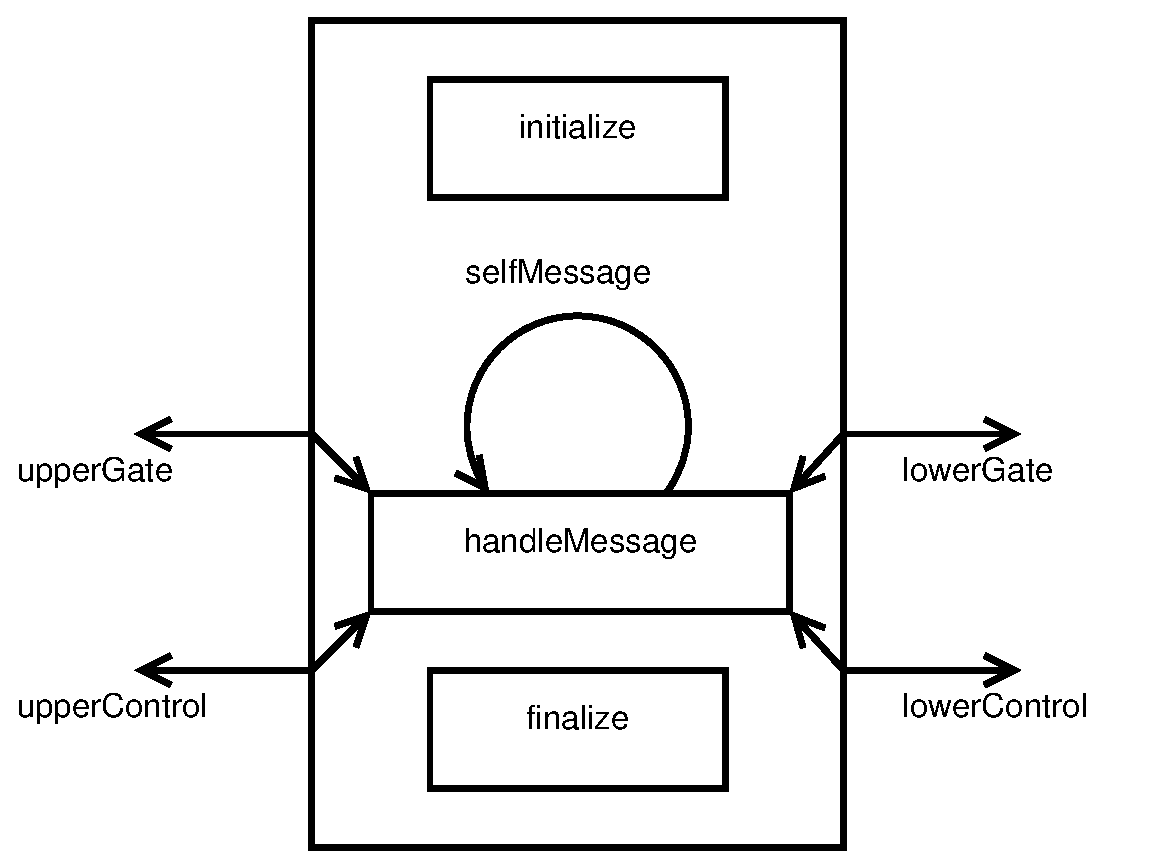
\includegraphics[width=0.5\textwidth]{omnetmodule.eps}
 \end{center}
 \caption{Basic \ac{OMNeT++} module structure}
 \label{fig:omnetmodule}
\end{figure}
 \item \textbf{sendDown/sendUp/sendControlDown/sendControlUp }This methods send a message from a module through the already commented gates.
 \item \textbf{scheduleAt - }This method schedules a self message in a certain time in the future. This is useful when programming timers or when a
message should be sent with a delay.
 \item \textbf{decapsMsg/encapsMsg - }Usually before a message is sent from one layer to another in the same device, it should be encapsulated or 
decapsulated. When this is done, instead of message, it is talked about packet. \textit{Packet} is a class that inherits from class \textit{message}. It 
is also possible to define a custom packet (check \cite{manualomnet} for this).
\end{itemize}

This methods and no others, were commented because they are going to be used many times during the work. For more information about \ac{OMNeT++}, 
refer to the user manual \cite{manualomnet}.

\subsection{\ac{MiXiM} Framework}

\ac{MiXiM} 2.0 framework provides \ac{OMNeT++} with many new modules. Among them, all necessary modules to work with 802.15.4 Standard. 
All this modules are build following \cite{IEEE802.15.4-2006}.

The basic structure of a node in \ac{MiXiM} is like shown in Figure \ref{fig:miximmodule}. This figure shows already some new modules added by
this work to the basic \ac{MiXiM} node. Depending on the kind of node: Computer, \ac{AN} or \ac{MN}, the \textit{.ned} files will load 
different modules to describe each behavior. This files should be also checked if a complete list of parameters is needed.

\begin{figure}[ht]
 \begin{center}
  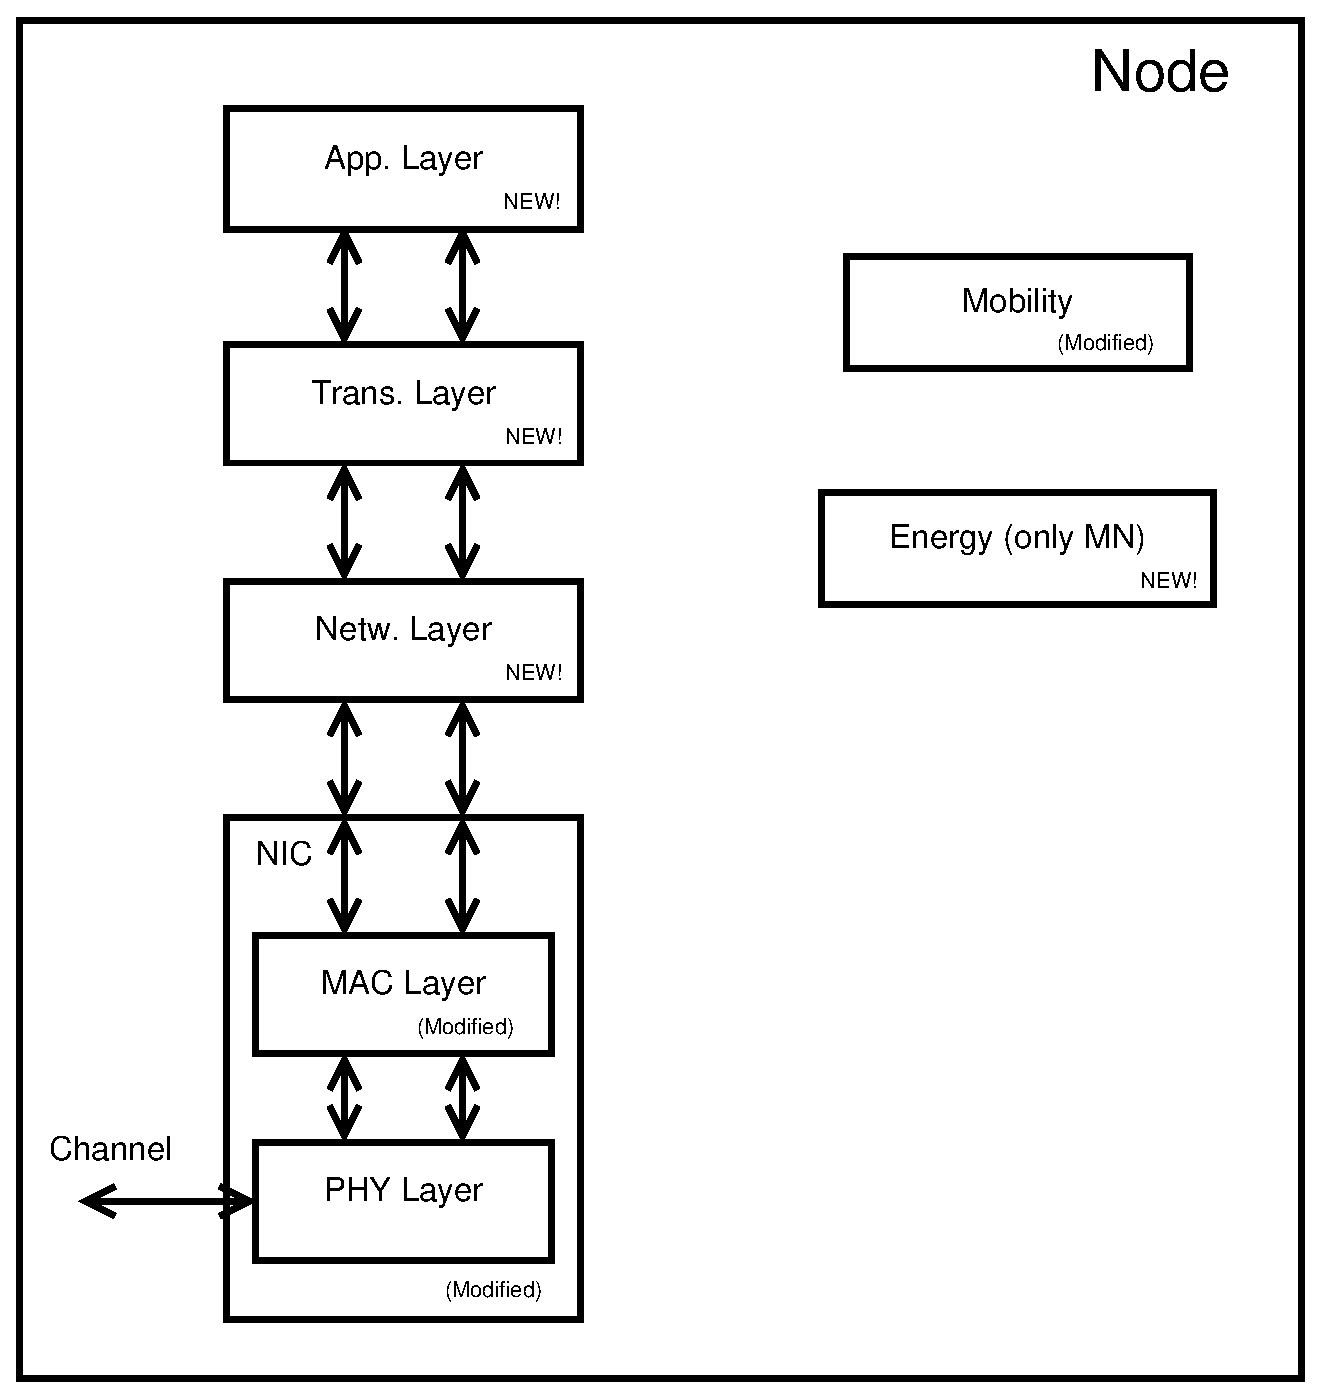
\includegraphics[width=0.8\textwidth]{miximmodule.eps}
 \end{center}
 \caption{Basic \ac{MiXiM} node structure}
 \label{fig:miximmodule}
\end{figure}

In this sub-section, only modified \ac{MiXiM} original modules will be commented leaving the new implemented modules for the next sub-sections.

\subsubsection{New packet structure}

In \ac{OMNeT++}, there are special files (\textit{.msg}) that define messages types. When the project is compiled, a class is automatically 
generated from every \textit{.msg} file. \ac{MiXiM} contributes \ac{OMNeT++} with many different message files. One of this files is the 
\textit{ApplPkt.msg}. This packet will be generated in the Application Layer and encapsulated in every layer until it gets transmitted into the 
air. For this work, this packet should include the following information that it did not before:
\begin{itemize}
 \item \textit{realDestAddr} and \textit{realSrcAddr}. This values are better explained with an example. When a \ac{MN} sends a report to the 
computer, the first step is sending the report to the selected \ac{AN}, this will be the \textit{destAddr} but the report is really intended
to go until the computer, this is the \textit{realDestAddr}. When this report arrives at the computer, for it, the \textit{srcAddr} is the 
address of the selected \ac{AN}, and the address of the \ac{MN} would be the \textit{realSrcAddr}.
 \item \textit{retransmisionCounterBO} and \textit{retransmisionCounterACK}. Whenever the \ac{MAC} Layer informs the Application Layer that a 
packet was dropped, Application Layer checks if there are still more retransmission available for this packet. Counter
\textit{retransmisionCounterBO} is used to check the case when packet was dropped due to a maximum number of Backoffs, and counter 
\textit{retransmisionCounterACK} is used to check the case where the packet was dropped because no \ac{ACK} was received. This counters are
increased by Applicaton Layer whenever a packet is retransmitted.
 \item \textit{CSMA}. This variable is a boolean, and if it is true, indicates the \ac{MAC} Layer that \ac{CSMA/CA} has to be disabled for 
this packet.
 \item \textit{askForRequest} and \textit{requestPacket}. This two variables are also booleans. When \textit{askForRequest} is true, it means
that \ac{MN} wants to notify the selected \ac{AN} that in the next period a data will be asked for. When \textit{requestPacket} is true, it
measn that \ac{MN} requests some information to the selected \ac{AN}. This flags are here to help the selected \ac{AN} to know what kind of 
report is receiving.
\end{itemize}

This packet structure is just for simulation purposes and has nothing to do with the real packet structure and hence with the size of the 
packet (\textit{bitLength} from \textit{cMessage} class) to be sent in the channel. Apart from Application Layer packet, \ac{MAC} and 
\ac{PHY} Layer will add their own headers. From Figure \ref{fig:MACFrame} on page~\pageref{fig:MACFrame} and Figure \ref{fig:PPDU} on 
page~\pageref{fig:PPDU} it is obtained that \ac{MAC} Layer header has 104 bits. And \ac{PHY} Layer header has 48 bits. This \ac{MAC} Layer
header size, assumes both addresses as short addressed, but in case a report has its origin or destination in a \ac{MN}, a long address 
must be used. This 6 bytes difference will be compensated adding them to Application Layer packet size.

According to Application Layer, the following real packets can be distinguished:
\begin{itemize}
 \item \underline{Sync Packet}. Has 1 byte for the status, 4 bytes for the next phase time-stamp and 2 + 2 + 2 bytes for \ac{AN} position. 
Its size is hence 88 bits.
 \item \underline{Normal Report}. Reports the listened \acp{RSSI} during the previous Sync Phases. It has 1 byte for the status and 2 bytes 
for each listened \ac{AN}. This report only exists for \acp{MN} in modes 1 and 4. As the source address is a \ac{MN}, 6 bytes have to be added.
Its size is hence $56 + 2\cdot X$ bits, where X is the number of \acp{AN} where a Sync Packet was listened to.
 \item \underline{\ac{MN} in mode 2 Report}. Reports the calculated positions from itself. It has 1 byte status and $2 + 2 + 2 = 6$ position 
bytes for each position calculated (maximum five). This report exists only for \acp{MN} in mode 2. As the source address is a \ac{MN}, 6 bytes 
have to be added. Its size is hence $56 + 6\cdot X$ bits, where X is the number of calculated positions to transmit.
 \item \underline{Ask Report}. Report or extra report with the ASK flag activated. In this case, 10 bytes are added to the report where the
flag is activated. This 10 bytes represent the information needed by the selected \ac{AN} to know which data the \ac{MN} is asking for.
 \item \underline{Request}. Report or extra report with the Request flag activated. In this case, 1 byte is added to the report where the
flag is activated. This byte shows which information was requested.
 \item \underline{\ac{MN}'s broadcast}. Broadcast packet sent by \acp{MN} in modes 3 and 4. It has 1 byte for the status and 1 byte information.
As the source address is a \ac{MN}, 6 bytes have to be added. Its size is hence 64 bits.
 \item \underline{\ac{AN}'s answer to request}. Report sent by \acp{AN} when answering a \ac{MN}'s request. It has 1 byte status and 10 bytes info.
As the destination address is a \ac{MN}, 6 bytes have to be added. Its size is hence 136 bits.
 \item \underline{Broadcasts collection packet}. Report sent by an \ac{AN} as collection of all broadcasts received from a \ac{MN} in mode 3 
or 4. It has 1 byte status, 2 bytes for \ac{RSSI} info and 6 bytes for showing which \ac{MN} the \ac{RSSI} belongs to. Its size is hence 72 bits.
\end{itemize}

\subsubsection{Connection Manager}

Apart from node structure modules, there is a central module in \ac{MiXiM}, called \textit{connectionManager}. This module is in charge of connecting
all nodes at a reachable distance. It keeps a list of all nodes and it is called every time a node changes its position. \textit{ConnectionManager} 
updates then the position in the list and recalculates all connections. The maximum distance where two nodes could still reach each other, is 
calculated using the transmit power and sensitivity, both are defined in \textit{omnetpp.ini}.

Each element from the node list is an object of the class \textit{NicEntry}. This class stores among many other data, the coordinates where the node is.
This class was modified to store also the following data:

\begin{itemize}
 \item \underline{Module Type}. It stores in the variable \textit{moduleType} the node type this \ac{NIC} belongs to. The values could be 1 for \ac{AN}, 
2 for \ac{MN} and 3 for Computer. Its value is assigned when initializing the node. As defining this variable here, it can be read from all modules in the 
network. This is useful to make lists of the different types of nodes.
 \item \underline{Slot Information}. Through variables \textit{transmisionSlot} and \textit{numSlots}, the \ac{AN} knows which slots of the 
\textit{numTotalSlots} are the ones reserved for it to transmit. All this three variables are assigned by the Computer in its \textit{initialize} method.
\end{itemize}

\subsubsection{Mobility module modifications}

The mobility module is the responsible of the node's positions. It is the one assigning the initial position to the nodes and it is also the one
used whenever a node wants to be moved. This module's functionality is described in class \textit{BaseMobility}. As the position of the nodes is needed,
this class is also linked with the \textit{NicEntry} class. Unlike \textit{connectionManager}, this is not a general module, and each node have their own
mobility node as it can be seen in Figure \ref{fig:miximmodule}.

During \textit{initialize} method in \textit{BaseMobility}, all node's initial positions, are assigned according to the values given in the file
\textit{omnetpp.ini}. A different value for each coordinate (X, Y, Z) must be given, and all of them must be inside the playground area (defined also
in \textit{omnetpp.ini}). When instead of a fixed value for the position, a ``-1'' is given, node will get a random position. The modifications done to
this class, refer precisely to the node's initial position assignment.

\begin{itemize}
 \item \underline{Uniform random distribution}. It was already seen that assigning ``-1'' as value for a node's coordinate, this coordinate will be 
randomly assigned. But if all coordinates are ``-1'', a new peace of code at \textit{stage} = 2 during \textit{initialize} method is executed. This 
code distributes \acp{AN} and \acp{MN} uniformly and randomly in the playground according to \textit{minimumDistanceAnchor} and 
\textit{minimumDistanceNode} parameter respectively. This two variables represent, as their names show, the minimum distance to leave among \acp{AN} 
and the minimum distance to leave among \acp{MN}.
 \item \underline{Grid distribution}. When ``-2'' is assigned to all \ac{AN}'s coordinate values in \textit{omnetpp.ini}, all \acp{AN} will be 
distributed all over the playground forming a grid. The dimensions of the grid will depend on the number of \acp{AN}, resulting for example for 25 
\acp{AN} a 5 x 5 grid. This grid distribution, will be done at \textit{stage} = 0 during \textit{initialize} method.
\end{itemize}

\subsubsection{\ac{MAC} Layer modifications}

\ac{MAC} Layer for 802.15.4 in \ac{MiXiM} is defined by the \textit{csma} class. This class works as a \ac{FSM} which diagram is as shown in Figure 
\ref{fig:csmaFSM}.

\begin{figure}[ht]
 \begin{center}
  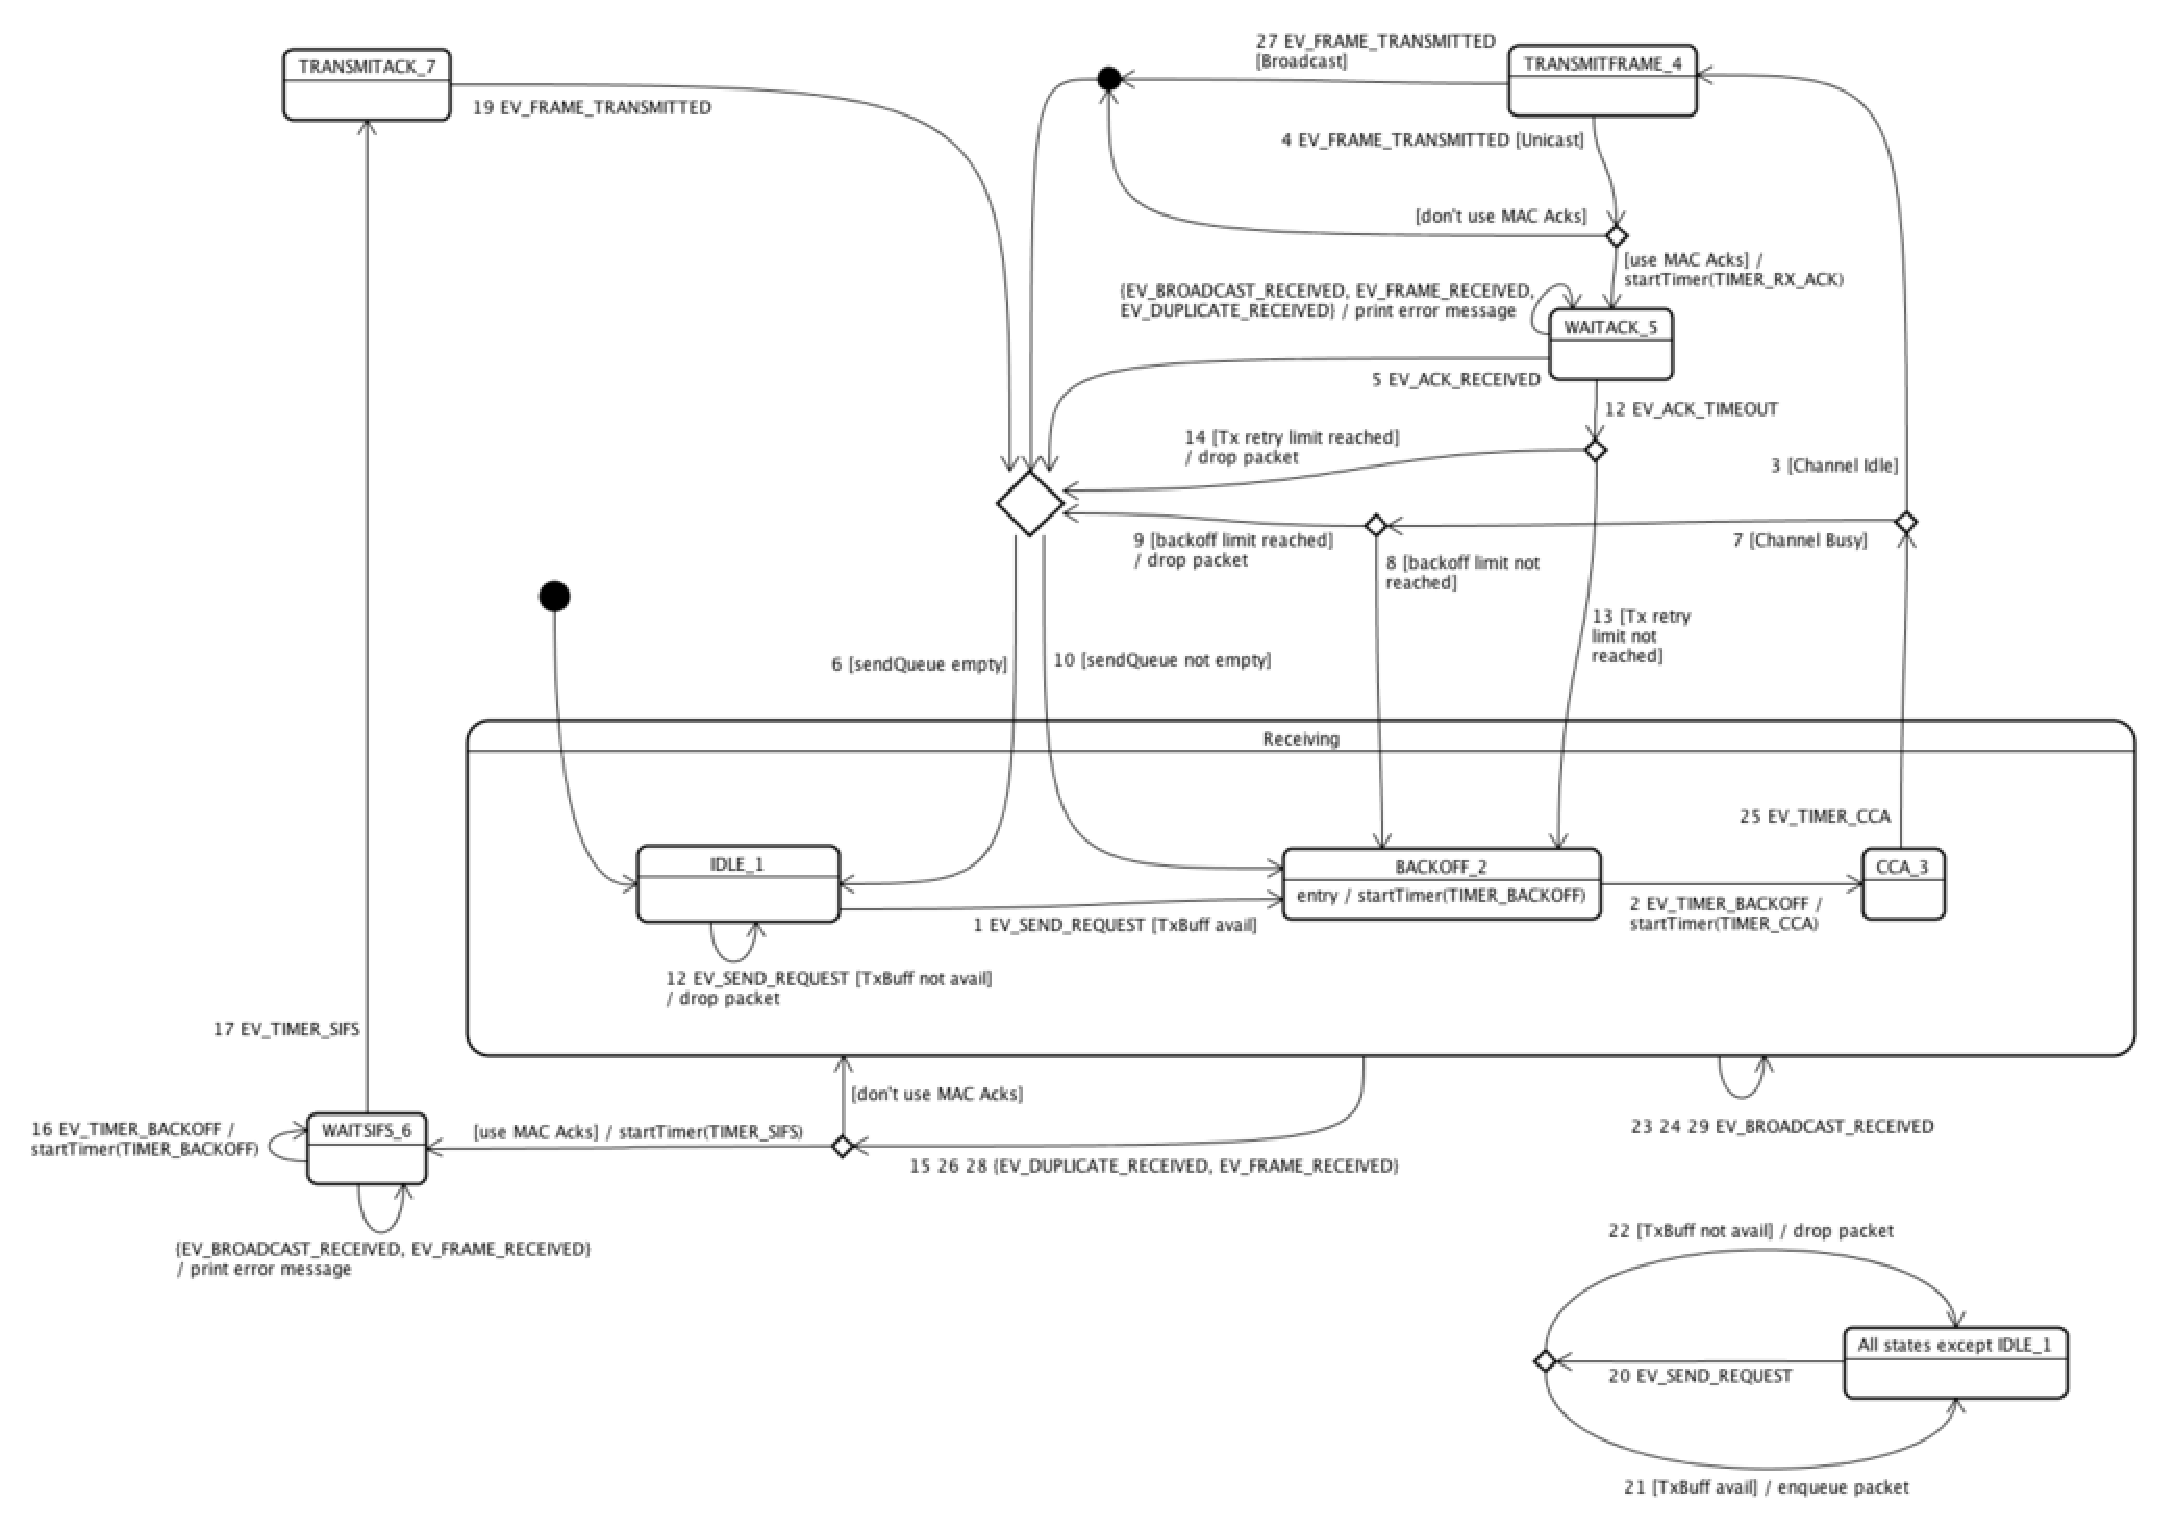
\includegraphics[width=1\textwidth]{csmaFSM.eps}
 \end{center}
 \caption{\ac{MiXiM}'s 802.15.4 \ac{MAC} Layer \ac{FSM} diagram \cite{MiXiM}}
 \label{fig:csmaFSM}
\end{figure}

Modifications done to this class are:

\begin{itemize}
 \item \underline{\ac{CSMA/CA} disable possibility}. During method \textit{updateStatusIdle} and whenever there is a packet in \ac{MAC} queue to
be transmitted, the first Backoff time would be calculated. In case the \ac{CSMA/CA} is deactivated, instead of calculating the first Backoff
time and scheduling the \ac{CCA} at this time, \ac{CCA} will be scheduled after \ac{SIFS} seconds (to assure Radio is in Rx state). If after the
\ac{CCA}, the channel is busy, the packet must be directly discarded instead of calculating a second Backoff time, that is why the \ac{NB} is 
set to the maximum number of retries. 
 \item \underline{Protocol phases end control}. It was added a way to control in which phase the node is, this control is started during the
\textit{initialize} method at stage 4 and it is rescheduled for every phase from method \textit{handleSelfMsg}. This control makes that the 
\ac{MAC} Layer, at the beginning from every phase, checks if the \ac{MAC} queue has elements from previous phase, in this case this elements
are erased and the number of elements recorded to have it as a result when calling the \textit{finish} method.

Before the end of every phase, it is left a \textit{guardTransmitTime} time. When \ac{MAC} Layer tries to send next packet in the queue, if the end of 
the first Backoff time goes beyond the guard time, this packet is not scheduled but it is erased. This erased packets number is also recorded
to be extracted as a result. This guard time for our work is 10 ms, it is this long to be protected even against the biggest packets during the 
simulation.
 \item \underline{Energy management}. In \ac{MiXiM}, although \ac{PHY} Layer has a SLEEP state, it is never used. This work has made \acp{MN}
going to sleep whenever they are able to. As this will be treated in Section \ref{sec:frameworkdevelopment} (\nameref{sec:frameworkdevelopment})
in a deeper way, here it would be just commented that whenever a \ac{MAC} state or a \ac{PHY} state gets changed in \textit{csma} class, another
class called \textit{energy} has to be warned.
 \item \underline{New control messages}. Before the modifications, \textit{csma} class informed upper layers whenever a sent report received an
\ac{ACK}, now, it informs also when broadcasts and \acp{ACK} were successfully sent to the channel. This class was also modified to 
report when a packet is dropped due to maximum number of Backoff retries, or to maximum number of ``no \ac{ACK} received`` retries, or when
\ac{MAC} Queue is full. Before it was only informing about packet dropped but without any reason. All this control messages will be treated 
in the Application Layer and they will be studied in following sections.
\end{itemize}

For a deeper view of \ac{MiXiM}'s \ac{MAC} Layer, a look up at \cite{MiXiM} and a deep view into the source code together with the diagram in Figure 
\ref{fig:csmaFSM} are recommended.


\section{Sync Phase study development}

Before constructing all the protocol framework, it had to be decided if during the Sync Phase the \acp{AN} would transmit their broadcasts 
synchronized in slots or randomly. For this purpose, a special and small framework was done, where just a simple Application Layer was added to 
the nodes. As this was just a temporary Application Layer, just the main aspects of it will be given.

\textit{Decider802154Narrow} class was modified to disable errors caused by noise and random errors due to the channel, this features were 
again enabled for the protocol framework development.

\subsection{\ac{MN}}

El nodo movil solo contaba el numero de paquetes recibidos en App

\subsection{Computer}

Solo calcula los slots

\subsection{\ac{AN}}

Los anchor generaban los paquetes de forma aleatoria esperando maximo 6 segundos (param definido en omnetpp.ini) y un maximo de paquetes tambien 
definido, o tambien los paquetes que les de tiempo en una segunda fase.

Cuando era con slots explicar el calculo de los slots y luego el tiempo que resultaba de este calculo para 3 veces por sync phase era el que se 
usaba en transmisiones aleatorias para ver cuantos paquetes daba tiempo en este tiempo.


\section{Framework development}
\label{sec:frameworkdevelopment}



Comentar que el routing es fijo para facilitarlo y hablar de la estructura de grid y del enrutamiento.
